%%% Please replace what is within each curly bracket with the correct information below. %%%
%%% The first field is already filled in for you.  %%%

\def\ClassName {COMP6600} % Your course 


\def\Answer{\textbf{Put your answer here:}}
\def\AnswerNoPrompt{}

%%COMMENT OUT TO PRODUCE BLANK DOCUMENT
\def \showSolutions{}

\documentclass[twoside]{article}
\usepackage{placeins}
\usepackage{class}
\usepackage{graphicx}
\graphicspath{{./figs/}}
\usepackage{amsmath, amsthm, amssymb}
\usepackage{url} 
\usepackage{enumerate}
\usepackage{wrapfig}
\usepackage{enumitem}
\usepackage{color}
\usepackage{pifont}
\usepackage{mdwlist}
\usepackage[lofdepth,lotdepth]{subfig}
\usepackage{mdwlist}
\usepackage[ampersand]{easylist}
\usepackage{wasysym}
\usepackage{tikz}

\usetikzlibrary{shapes.geometric}
\usetikzlibrary{positioning}

\ListProperties(Hide=100, Hang=true, Progressive=3ex, Style*=-- ,
Style2*=$\bullet$ ,Style3*=$\circ$ ,Style4*=\tiny$\blacksquare$ )
\title{HW2}
\usepackage{multirow}

\pagestyle{myheadings}

\renewcommand{\P}{\mathbf{P}}
\newcommand{\eat}[1]{\ignorespaces}
\newcommand{\todo}[1]{ {\color{blue} TODO: #1} }
\newcommand{\X}{\ding{110}}
\newcommand{\F}{$\bullet$}
\newcommand{\Pac}{$<$}
\newcommand{\bigCI}{\mathrel{\text{\scalebox{1.07}{$\perp\mkern-10mu\perp$}}}}
\def\truefalse{\vspace{0.3in} \item (\emph{true} or \emph{false}) }
\def\indep{\perp\!\!\!\perp}
\def\sgn{\mathop{\mathrm{sign}}}
\newcommand{\solutionspace}[4]{\fbox{\begin{minipage}[t][#1][t]{#2} \textbf{#3} 

\solution{}{#4} \end{minipage}}}

% Bubbles for multiple choice questions
\newcommand{\emptycircle}{$\Large\bigcirc$}
\newcommand{\filledcircle}{$\Large\newmoon$}
\newcommand{\mcqb}{$\bigcirc$\ \ }
\newcommand{\mcqs}{\solution{\mcqb}{$\Large\newmoon$\ \ }}
\newcommand{\emptysquare}{{\Large $\square$}\ \ }
\newcommand{\filledsquare}{{\Large $\boxtimes$}\ \ }
\newcommand{\squaresolution}{\solution{\emptysquare}{\filledsquare}}


\begin{document}
\thispagestyle{empty}

\def\Name {}  % Your name
\def\AuburnID{} % Your AuburnID

\def\TwoHours{    
    \emptycircle
    % \filledcircle
} 
\def\FourHours{    
    \emptycircle
    % \filledcircle
} 
\def\SixHours{    
    \emptycircle
    % \filledcircle
} 
\def\EightHours{    
    \emptycircle
    % \filledcircle
} 
\def\MoreThanEightHours{    
    \emptycircle
    % \filledcircle
} 


%%%%%%%%%%%%%%%%%%%%%%%%%%%%%%%%%%%%%%%%%%%%%%%%%%%
%%%%%%%%%%%%%%%%%%%% Problem 1 %%%%%%%%%%%%%%%%%%%%
%%%%%%%%%%%%%%%%%%%%%%%%%%%%%%%%%%%%%%%%%%%%%%%%%%%

\def \Oneb{x}
%%%%%%%%%%%%%%%%%%%%%%%%%%%%%%%%%%%%%%%%%%%%%%%%%%%
%%%%%%%%%%%%%%%%%%%% Problem 2 %%%%%%%%%%%%%%%%%%%%
%%%%%%%%%%%%%%%%%%%%%%%%%%%%%%%%%%%%%%%%%%%%%%%%%%%

\def \Twob{x}

%%%%%%%%%%%%%%%%%%%%%%%%%%%%%%%%%%%%%%%%%%%%%%%%%%%
%%%%%%%%%%%%%%%%%%%% Problem 3 %%%%%%%%%%%%%%%%%%%%
%%%%%%%%%%%%%%%%%%%%%%%%%%%%%%%%%%%%%%%%%%%%%%%%%%%
\def \Threea{x}

\def \Threeb{x}

%%%%%%%%%%%%%%%%%%%%%%%%%%%%%%%%%%%%%%%%%%%%%%%%%%%
%%%%%%%%%%%%%%%%%%%% Problem 4 %%%%%%%%%%%%%%%%%%%%
%%%%%%%%%%%%%%%%%%%%%%%%%%%%%%%%%%%%%%%%%%%%%%%%%%%
\def \Foura{x}

\def \Fourb{x}

\def \Fourc{x}

%%%%%%%%%%%%%%%%%%%%%%%%%%%%%%%%%%%%%%%%%%%%%%%%%%%
%%%%%%%%%%%%%%%%%%%% Problem 5 %%%%%%%%%%%%%%%%%%%%
%%%%%%%%%%%%%%%%%%%%%%%%%%%%%%%%%%%%%%%%%%%%%%%%%%%
\def \Fiveai{x}
\def \Fiveaii{x}
\def \Fiveaiii{x}
\def \Fiveaiv{x}


\def \Fivebi{y}
\def \Fivebii{y}
\def \Fivebiii{y}
\def \Fivebiv{y}


\def\Fiveci{y}
\def\Fivecii{y}
\def\Fiveciii{y}
\def\Fiveciv{y}
\def\Fivecv{y}
\def\Fivecvi{y}
\def\Fivecvii{y}
\def\Fivecviii{y}
\def\Fivecix{y}
\def\Fivecx{y}

\def\Fivedi{y}
\def\Fivedii{y}
%%%%%%%%%%%%%%%%%%%%%%%%%%%%%%%%%%%%%%%%%%%%%%%%%%%%%%%%
%%%%%%%%%%%%%%%%%%%% STAFF USE ONLY %%%%%%%%%%%%%%%%%%%%
%%%%%%%%%%%%%%%%%%%%%%%%%%%%%%%%%%%%%%%%%%%%%%%%%%%%%%%%

%% You don't need to fill out the following, only for grading purposes
\def \OneGReason{}
\def \OneHReason{}
\def \OneIReason{}
\def \ThreeCAdmissibleReason{}
\def \ThreeCConsistentReason{}
\def \ThreeDAdmissibleReason{}
\def \ThreeDConsistentReason{}
\def \FourAAReason{}
\def \FourABReason{}
\def \FourACReason{}
\def \FourADReason{}
\def \FourAEReason{}
\def \FourAFReason{}
\def \FourBReason{}

%
%                                  Y\     /Y
%                                  | \ _ / |
%            _____                 | =(_)= |
%        ,-~"     "~-.           ,-~\/^ ^\/~-.
%      ,^ ___     ___ ^.       ,^ ___     ___ ^.
%     / .^   ^. .^   ^. \     / .^   ^. .^   ^. \
%    Y  l    O! l    O!  Y   Y  lo    ! lo    !  Y
%    l_ `.___.' `.___.' _[   l_ `.___.' `.___.' _[
%    l^~"-------------"~^I   l^~"-------------"~^I
%    !\,               ,/!   !                   !
%     \ ~-.,_______,.-~ /     \                 /
%      ^.             .^       ^.             .^  
%        "-.._____.,-"           "-.._____.,-"
%

\maketitle 
\smallskip
\smallskip
\textbf{INSTRUCTIONS}

\begin{itemize}
\item \textbf{Due:} \textbf{Sunday, 2 March 2025 at 11:59 PM CST.} 
\item \textbf{Format:} Write your answers in the \texttt{yoursolution.tex} file and latex a pdf (preferred) or you can type directly on the blank pdf. Make sure that your answers are within the dedicated regions for each question/part. If you do not follow this format, we may deduct points. 
% You may use digital tools (e.g., an iPad) to handwrite your solutions, but make sure they are legible.
% We reserve the right to take points off if we can't read your solution. 
\item \textbf{Images:} To insert pictures, we recommend drawing it on PowerPoint or Google Drawings, saving it as an image and including it in your latex source.

\item Please use \LaTeX\ to produce your writeups. For these problems the easiest way to "write" your solutions is probably to download all image files, insert them into a google slide deck, then insert text to write your answers, export as a png and put that in your latex write-up.

\item \textbf{How to submit:} Submit a pdf with your answers on Canvas. Log in and click on our class 5600/6600 and click on the submission titled Homework 1 and upload your pdf containing your answers. 
\item \textbf{Policy:} See the course website for homework policies and Academic Integrity.

\end{itemize}

\begin{center}
\begin{tabular}{|r|c|}
\hline
\begin{minipage}{3cm}~\\Name~\\~\\\end{minipage} & \begin{minipage}[c][1cm][c]{8cm} ~ \Name \end{minipage}  \\
\hline
\begin{minipage}{3cm}~\\Auburn ID~\\~\\\end{minipage} & \AuburnID \\
\hline
\begin{minipage}{3cm}~\\Hours to complete? ~\\\end{minipage} & \solution{\emptycircle}{\TwoHours} (0, 2] hours \hspace{0.5cm} \solution{\emptycircle}{\FourHours} (2, 4] hours \hspace{0.5cm}
\solution{\emptycircle}{\SixHours} (4, 6] hours \hspace{0.5cm} \\
&
\solution{\emptycircle}{\EightHours} (6, 8] hours \hspace{0.5cm}
\solution{\emptycircle}{\MoreThanEightHours} $>$ 8 hours \\
\hline

\end{tabular}
\end{center}



\vfill

\smallskip
\smallskip
\smallskip
\smallskip
\smallskip

\begin{center}
{\bf For TA use only}\\
\begin{Large}
\begin{tabular}{|r|r|r|r|r|r|r|r|}
\hline
Q1 & Q2 & Q3 & Q4 & Q5 & Total \\
\hline
\quad/15 &\quad/20 & \quad/20 & \quad/24 &\quad/21 & \quad/100 \\
\hline
\end{tabular}\end{Large}
\end{center}


\newpage



\begin{problem} {Search and Heuristics}

\begin{question}[10] For the following game tree, carry out minimax search. Give the value for each node.

\begin{center}
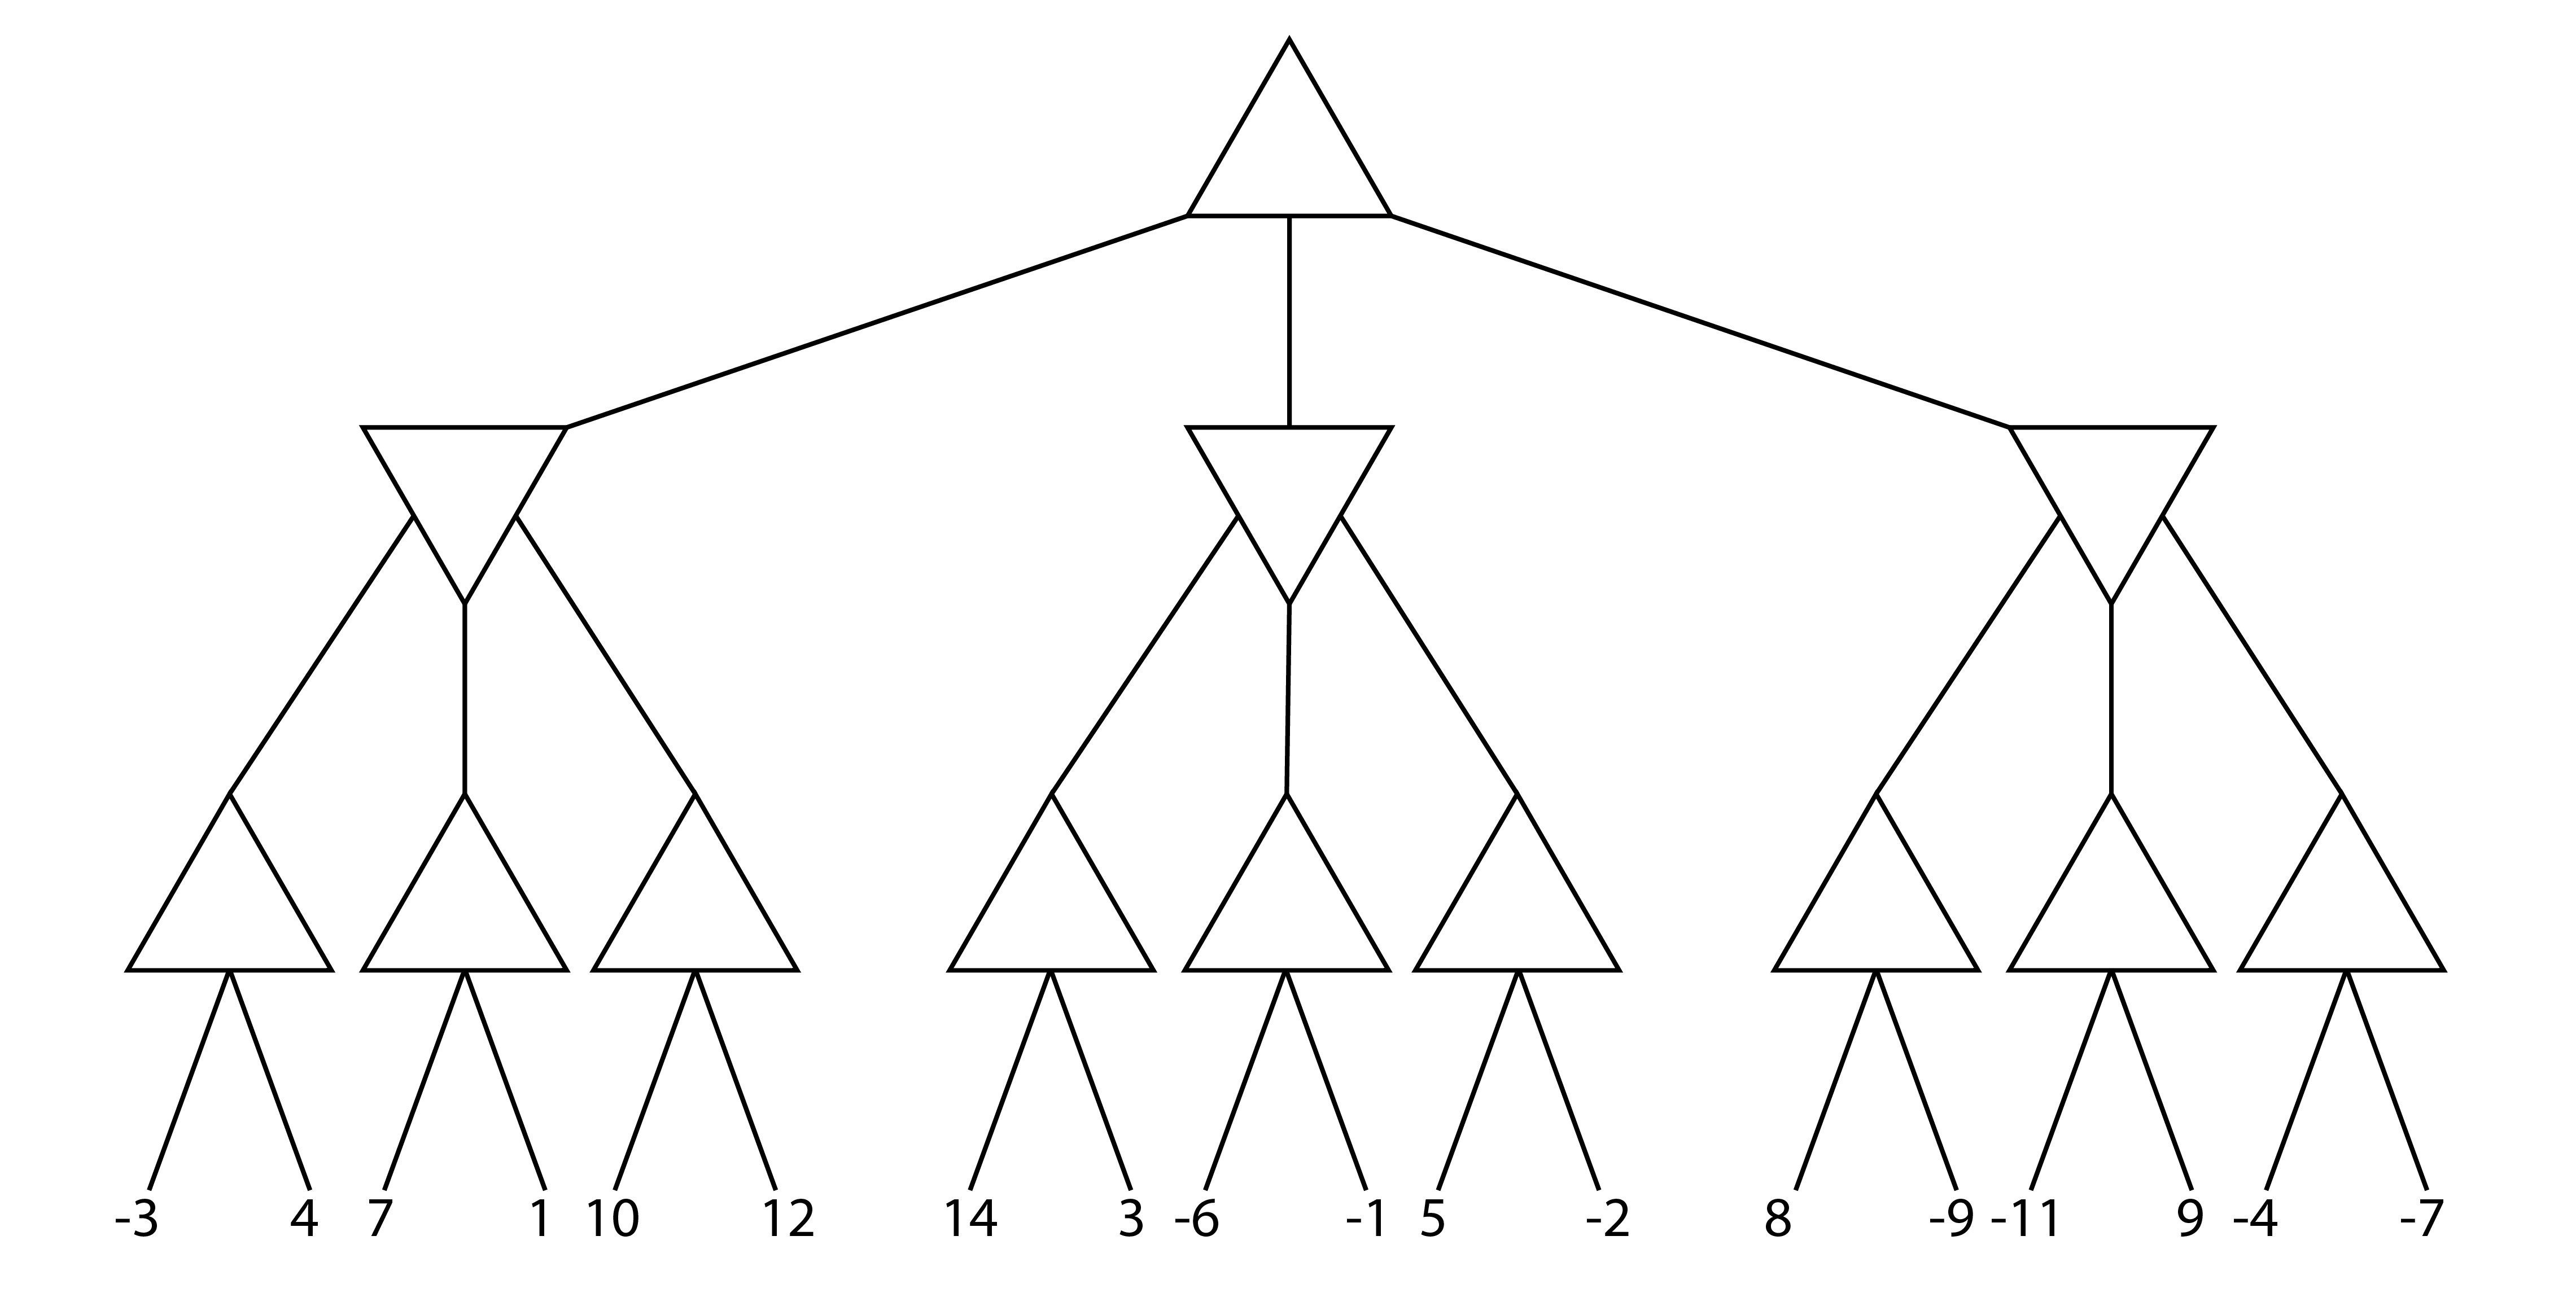
\includegraphics[width=\linewidth]{gametree.png}
\end{center}

\end{question}

\begin{question}[5] What move should you make now? How much is the game worth to you?

\solutionspace{2cm}{15cm}{}
{\Oneb}

\end{question}

\end{problem}

\clearpage
\begin{problem} {Alpha-Beta pruning}

\begin{question} [10] For the same game tree perform alpha-beta pruning. Let $(\alpha, \beta)_{i}$ be the
  $\alpha$-$\beta$ values passed down an edge to node $i$.  Similarly,
  $v_i$ is the value passed up edge $i$, etc..  Show the sequence of
  steps, by giving the $(\alpha, \beta)$ values on the way down, and the $v$ values
  on the way up. 

\begin{center}
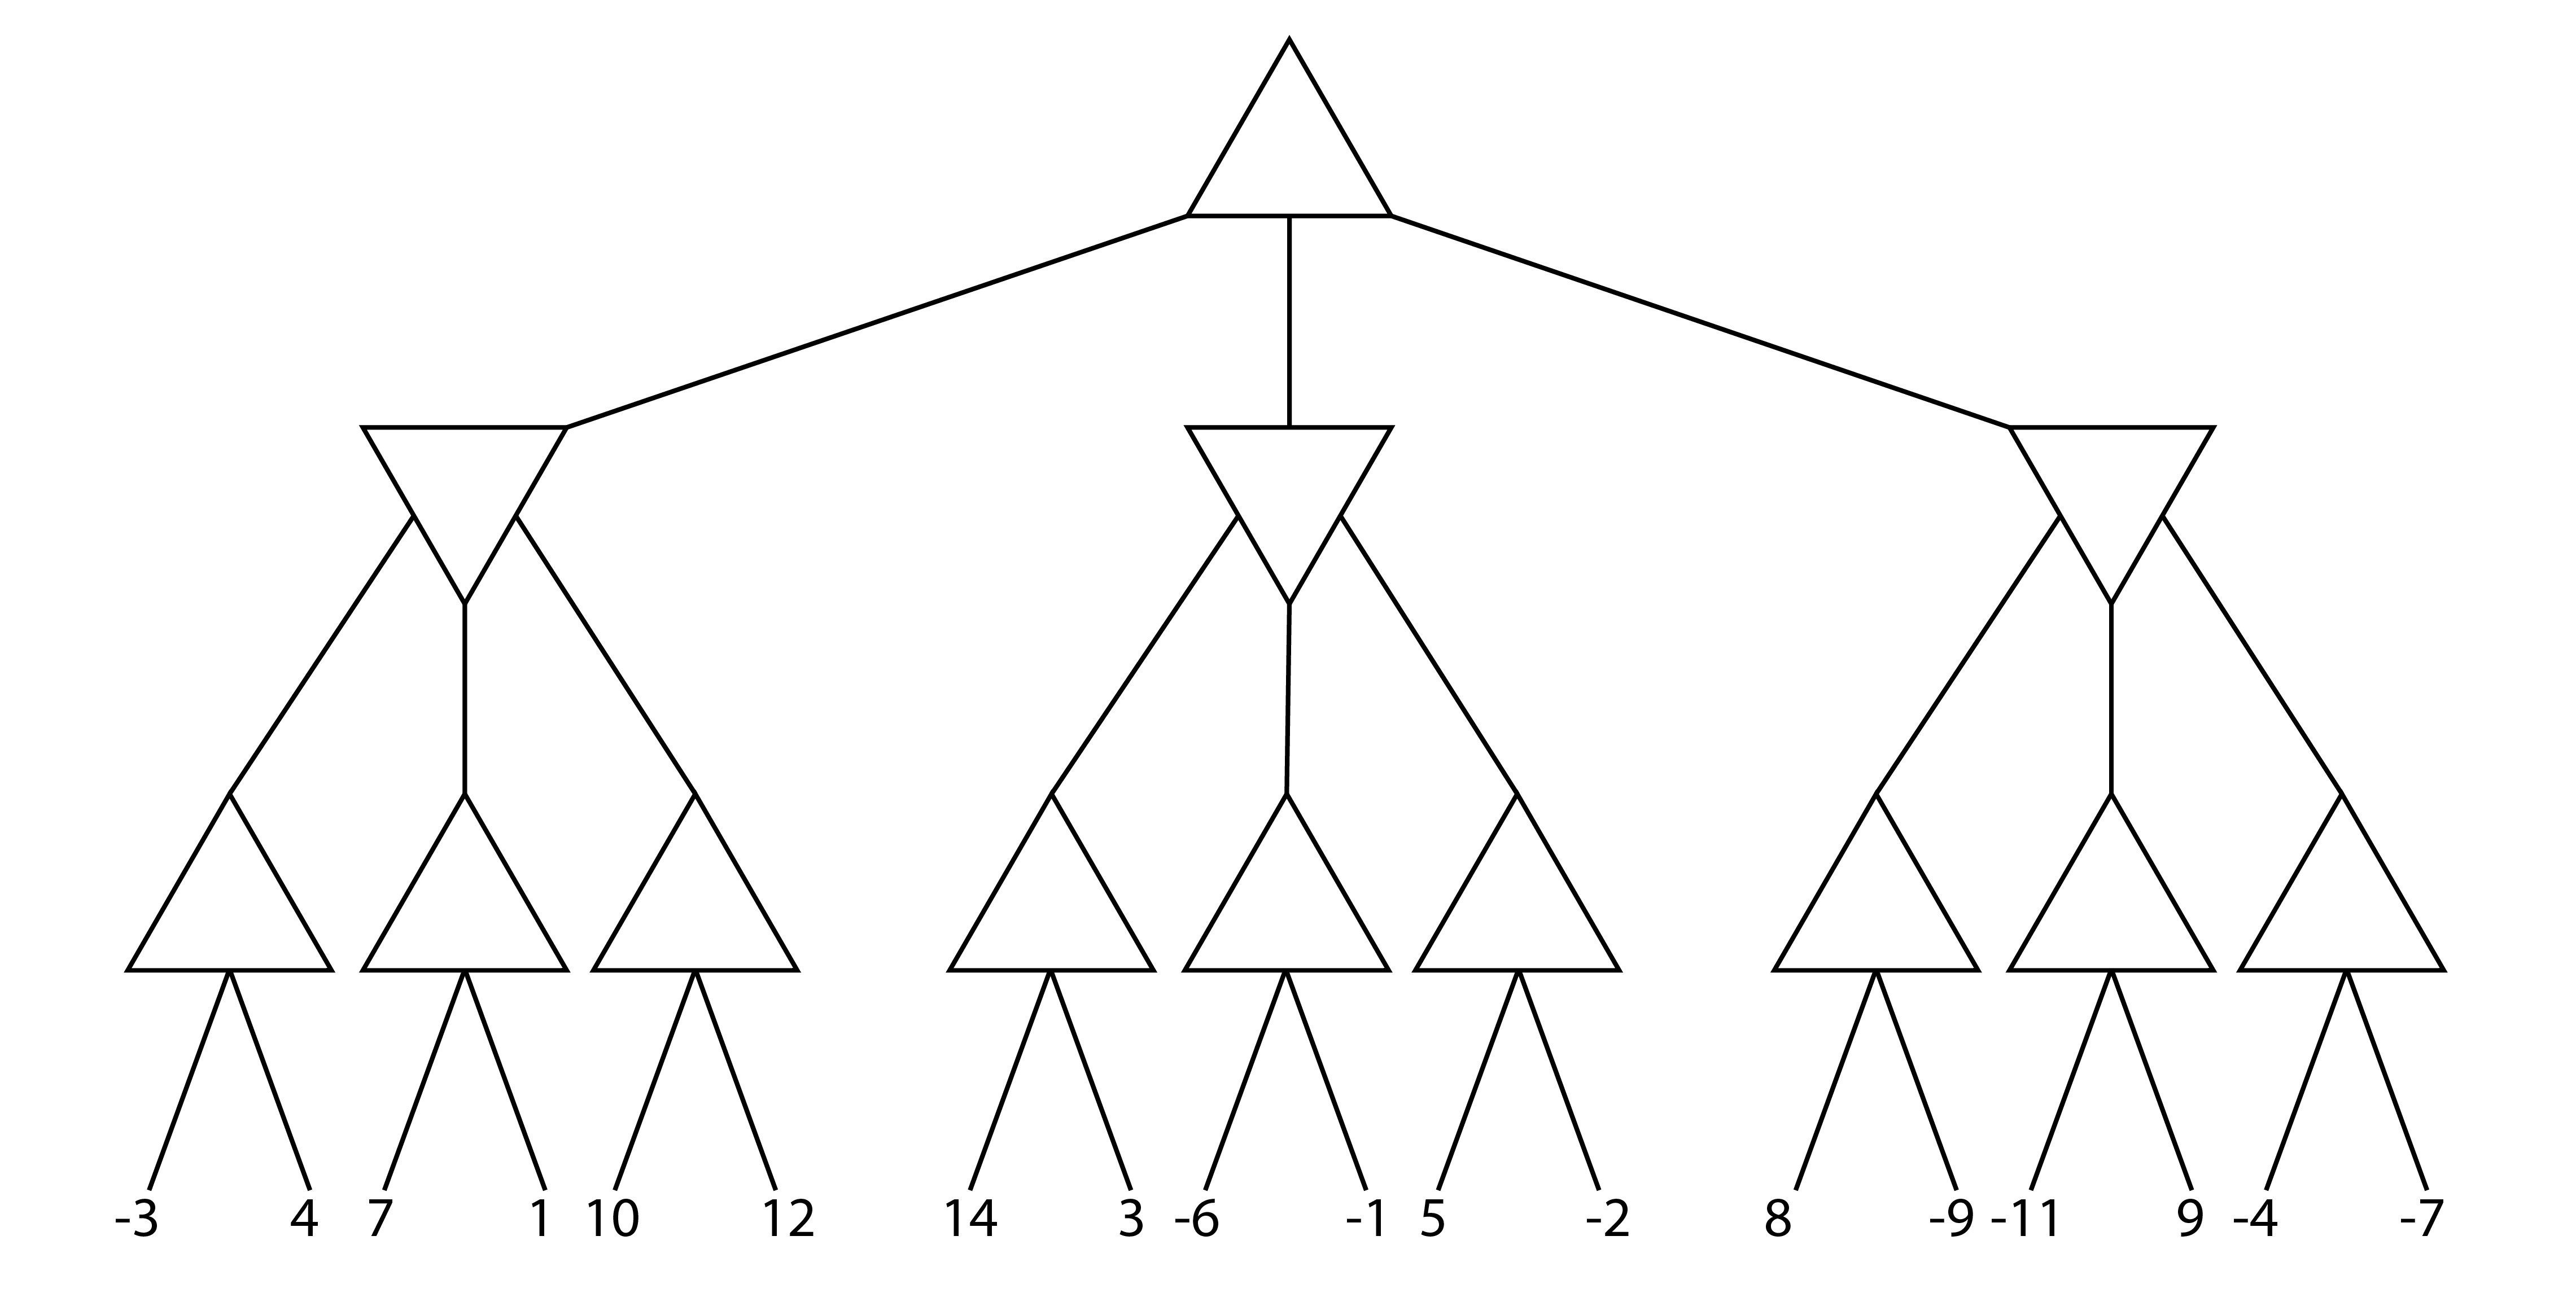
\includegraphics[width=\linewidth]{gametree.png}
\end{center}
\end{question}

\begin{question} [10]  Which leaf nodes are never visited due to pruning?

\solutionspace{2cm}{15cm}{}
{\Twob}

\end{question}

\end{problem}


\begin{problem} {Expectimax}

Consider the zero-sum expectimax game tree below.  Circles represent
chance nodes.  Trapezoids that point up represent choices for the
player seeking to maximize. Outcome values for the maximizing player
are listed for each leaf node.

\begin{question}[10] First, assume that each chance node chooses uniformly between
  available moves. Assuming optimal play, carry out the expectimax
  search algorithm and write the value of each node inside the
  corresponding trapezoid. What is the expected value of this game
  assuming optimal play? What is the optimal move to make at each
  node?  Fill in the node values using a drawing program.

\begin{center}
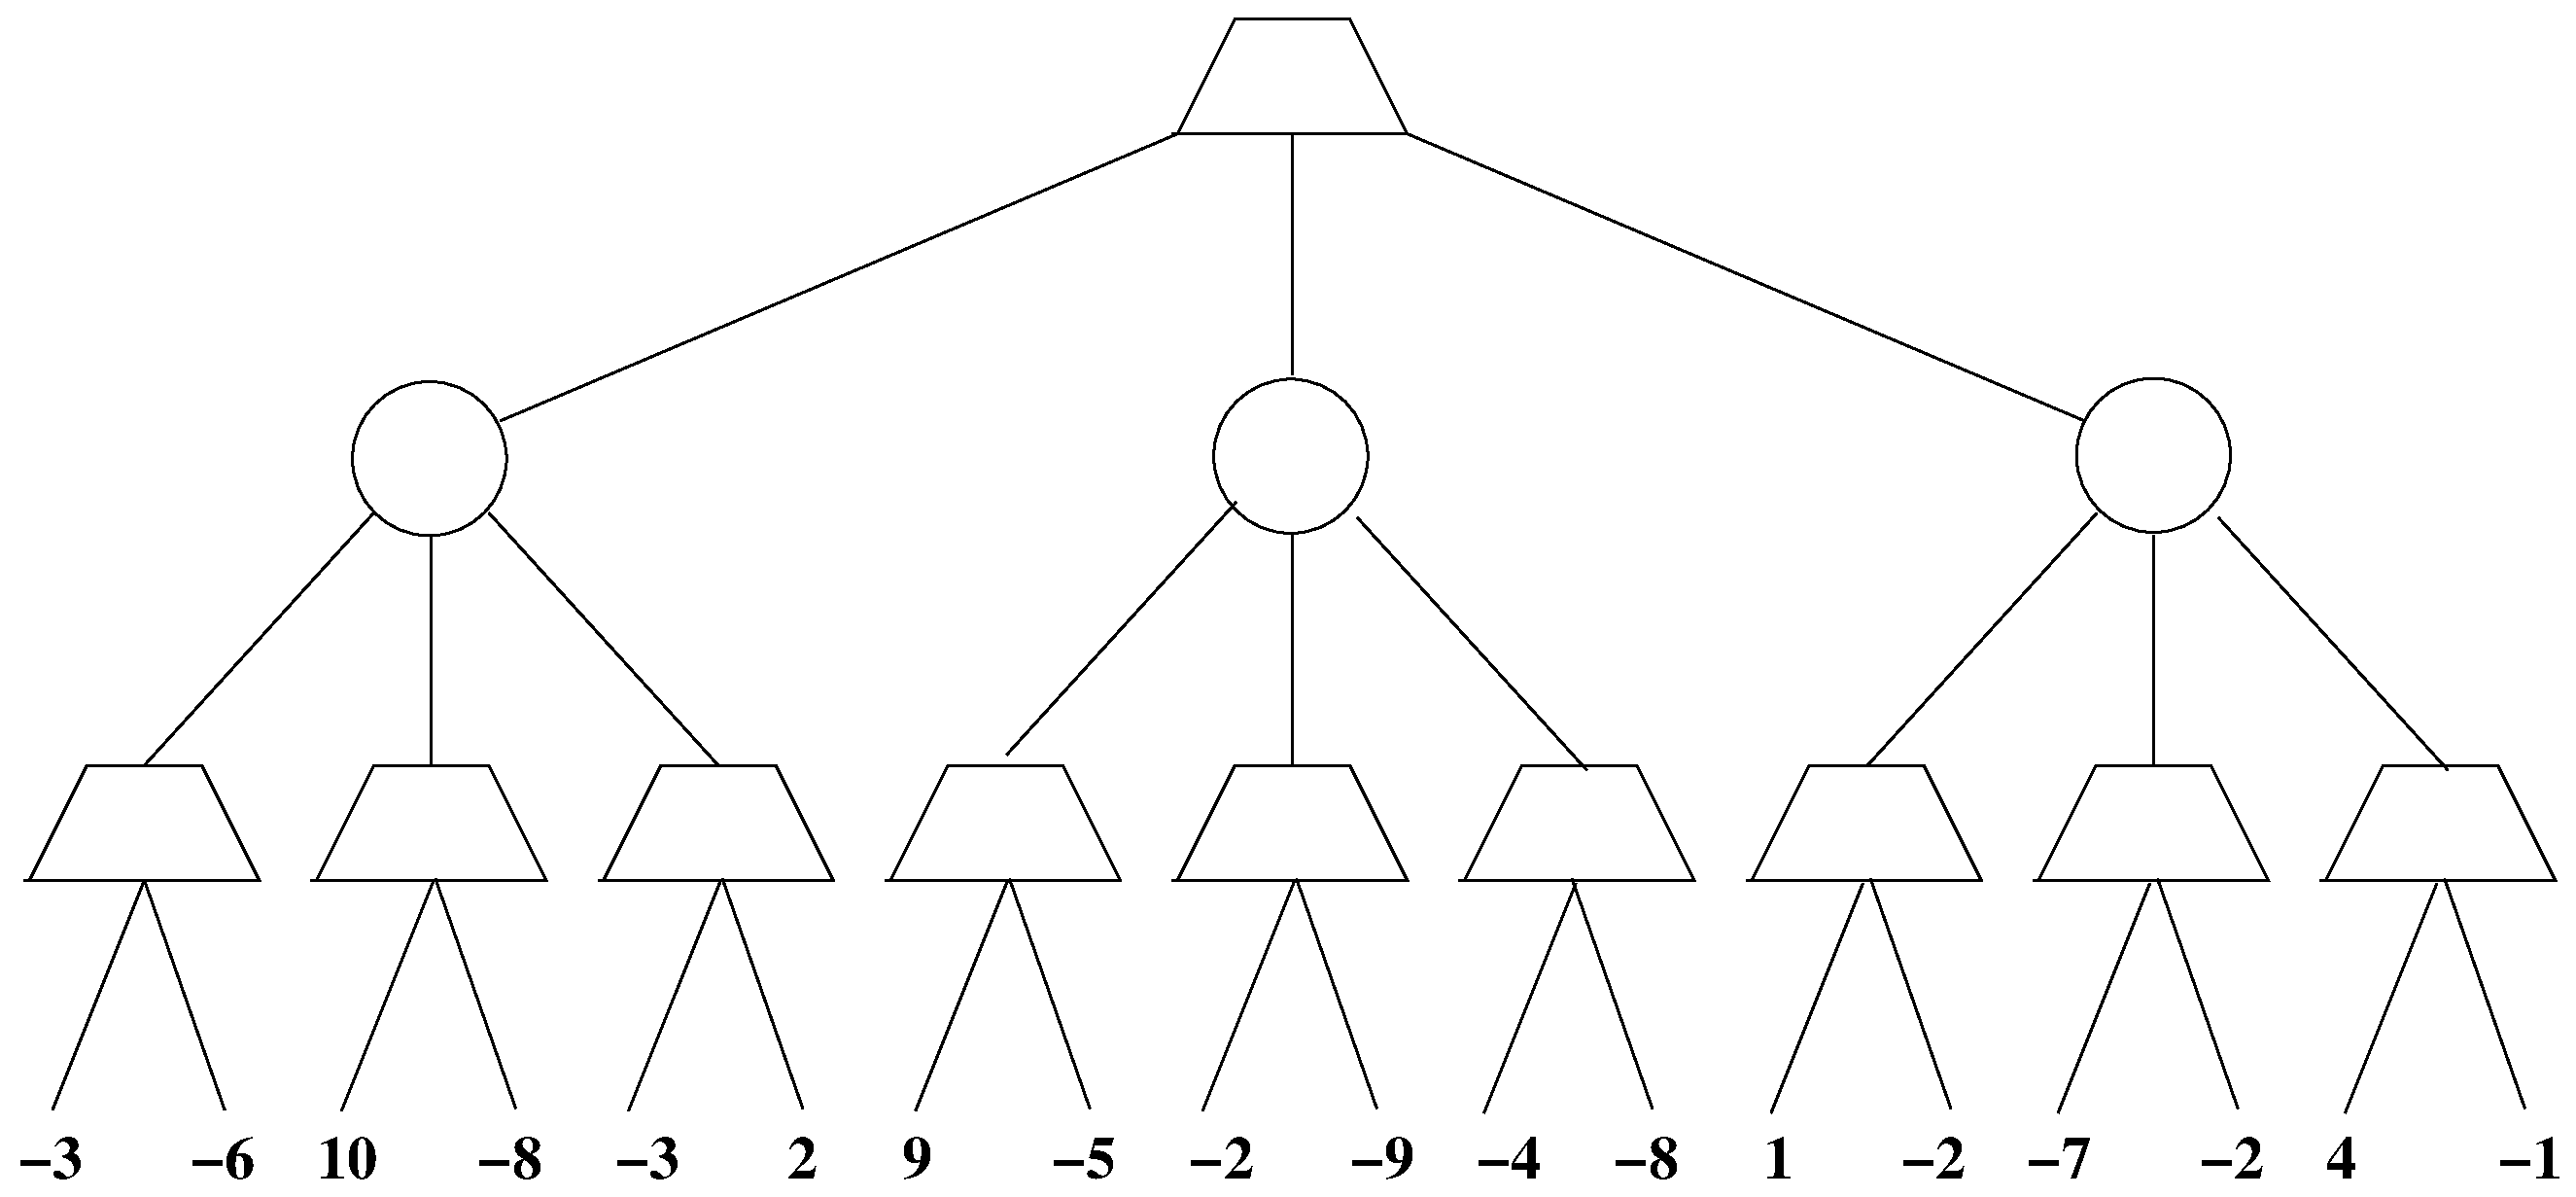
\includegraphics[width=6in]{expectimax.eps}
\end{center}

\solutionspace{1cm}{15cm}{}
{\Threea}


\end{question}


\begin{question}[10] Now, assume that each chance node plays the leftmost move with
  probability 0.5, the middle move with probability 0.25, and the
  rightmost move with probability 0.25. Assuming optimal play, what is
  the expected value of this game?  What is the optimal move to make?
  Fill in the node values using a drawing program.

\begin{center}
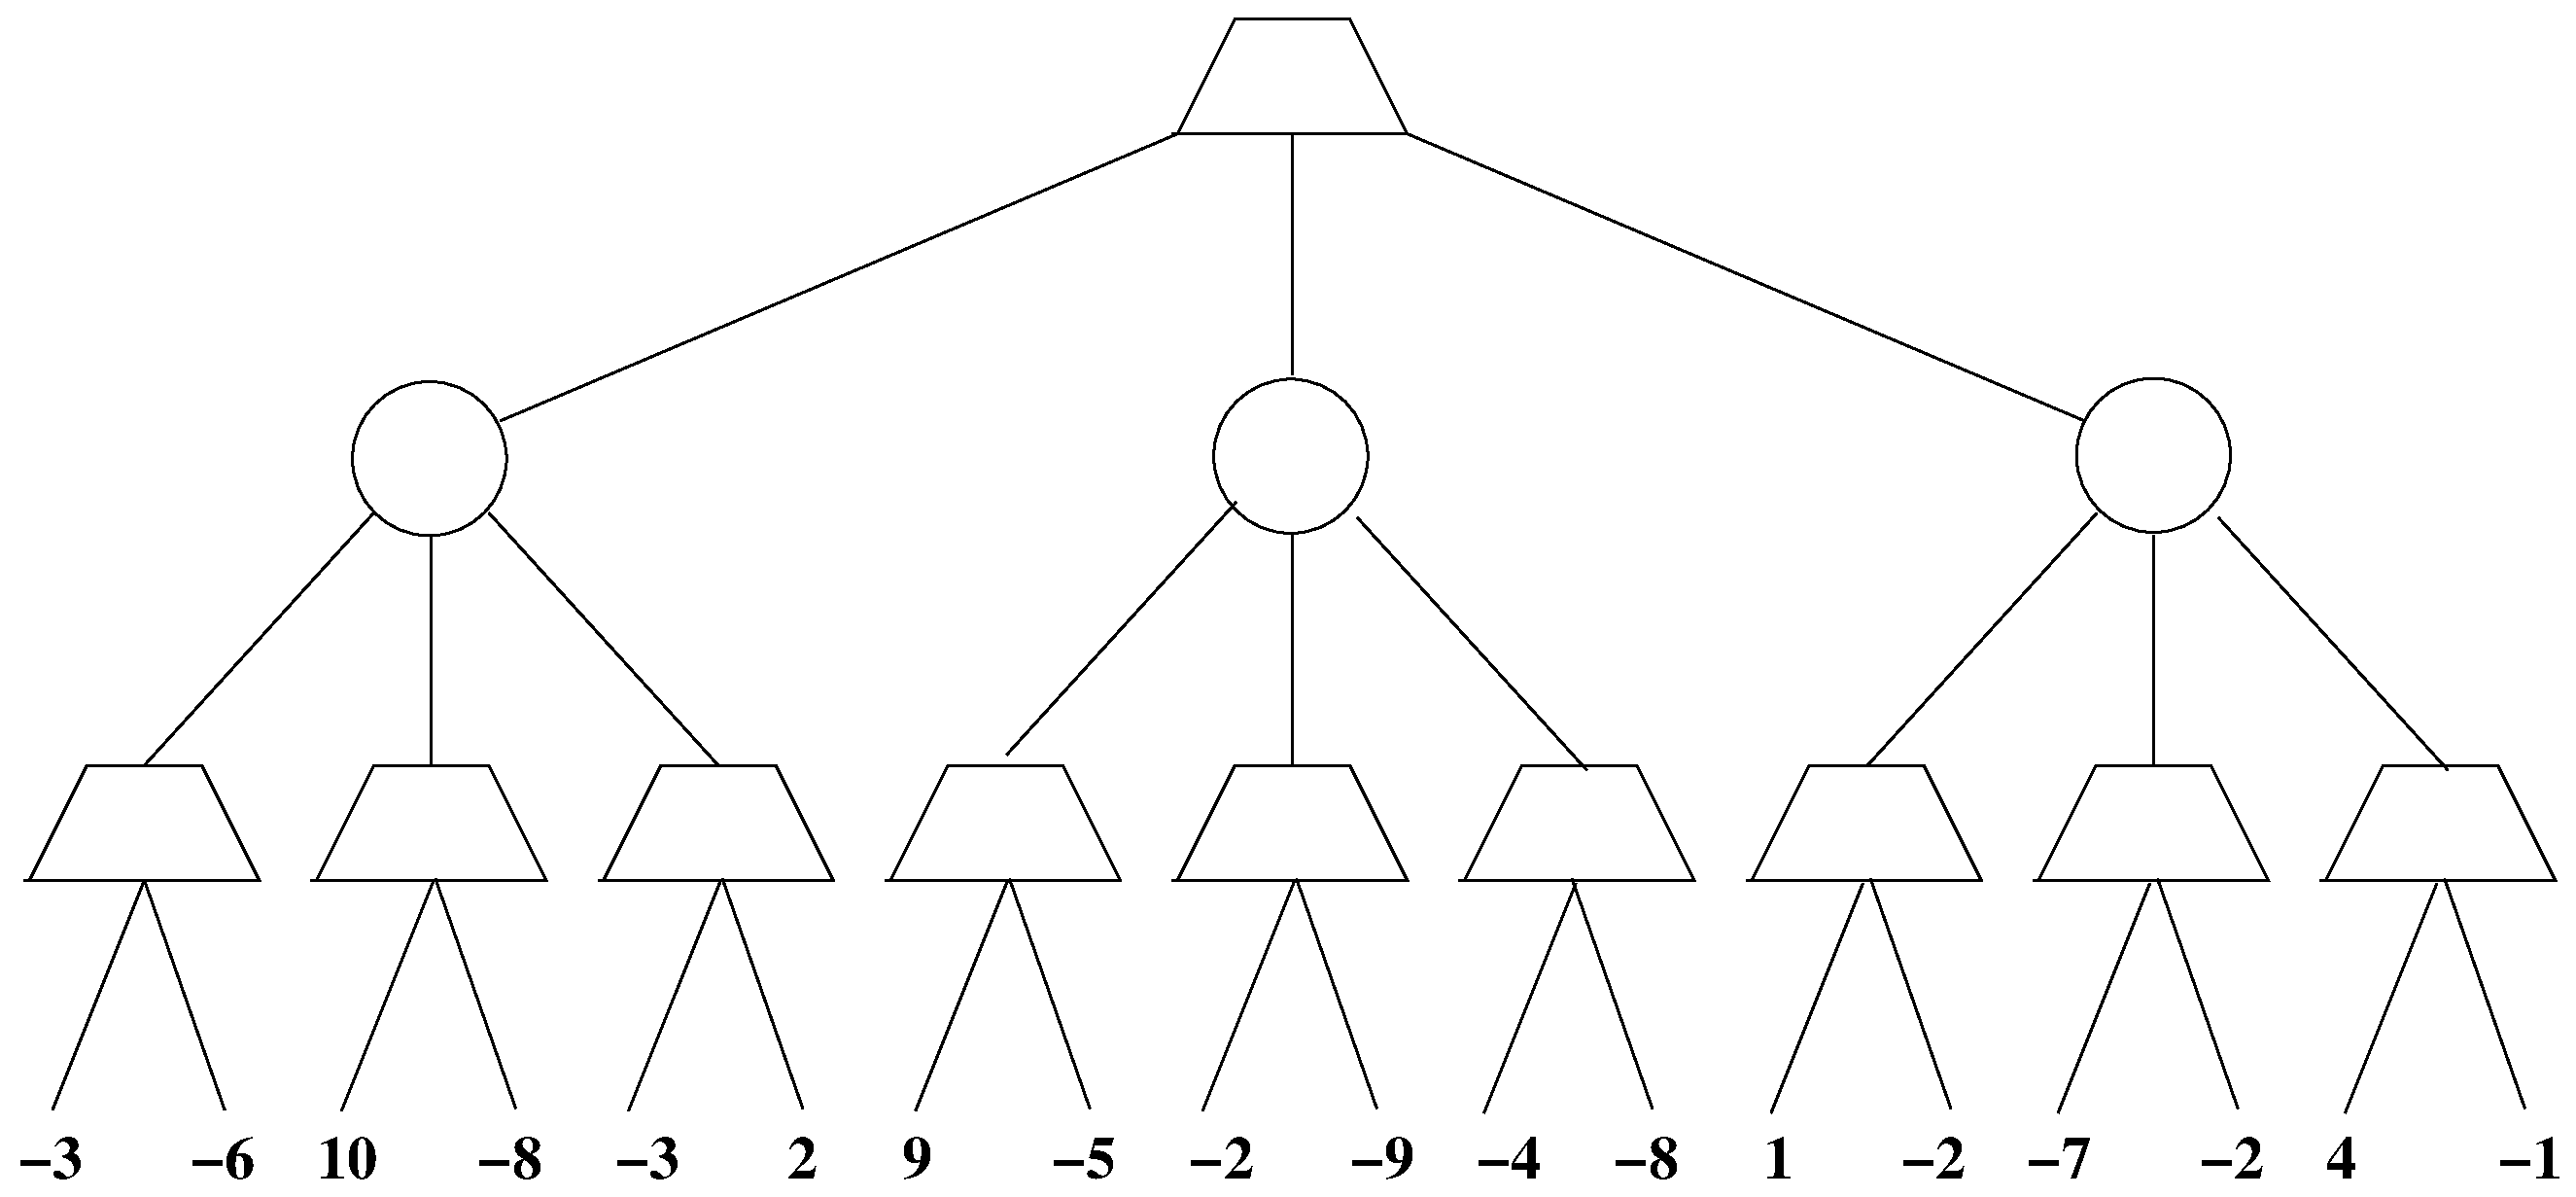
\includegraphics[width=6in]{expectimax.eps}
\end{center}

\solutionspace{1cm}{15cm}{}
{\Threeb}


\end{question}

\end{problem}

\clearpage

\begin{problem}{Alpha Beta Expinimax}
In this question, Player A acts as a minimizer, Player B as a maximizer, and C represents a chance node. Each child of a chance node occurs with equal probability. The game tree consists of players A, B, and C, incorporating both deterministic and stochastic elements. In lecture, we explored pruning in Minimax game trees. In this question, you will analyze Expectimax pruning—a similar approach but incorporating chance nodes. Assume that nodes are visited from left to right. For each of the following game trees, give an assignment of terminal values to the leaf nodes such that the bolded node can be pruned (it doesn’t matter if you prune more nodes), or write “not possible” if no such
assignment exists. You may give an assignment where an ancestor of the bolded node is pruned (since then
the bolded node will never be visited). You should not prune on equality, and your terminal values must be
finite (including negative values).

\begin{question}[8] Game Tree 1

\begin{center}
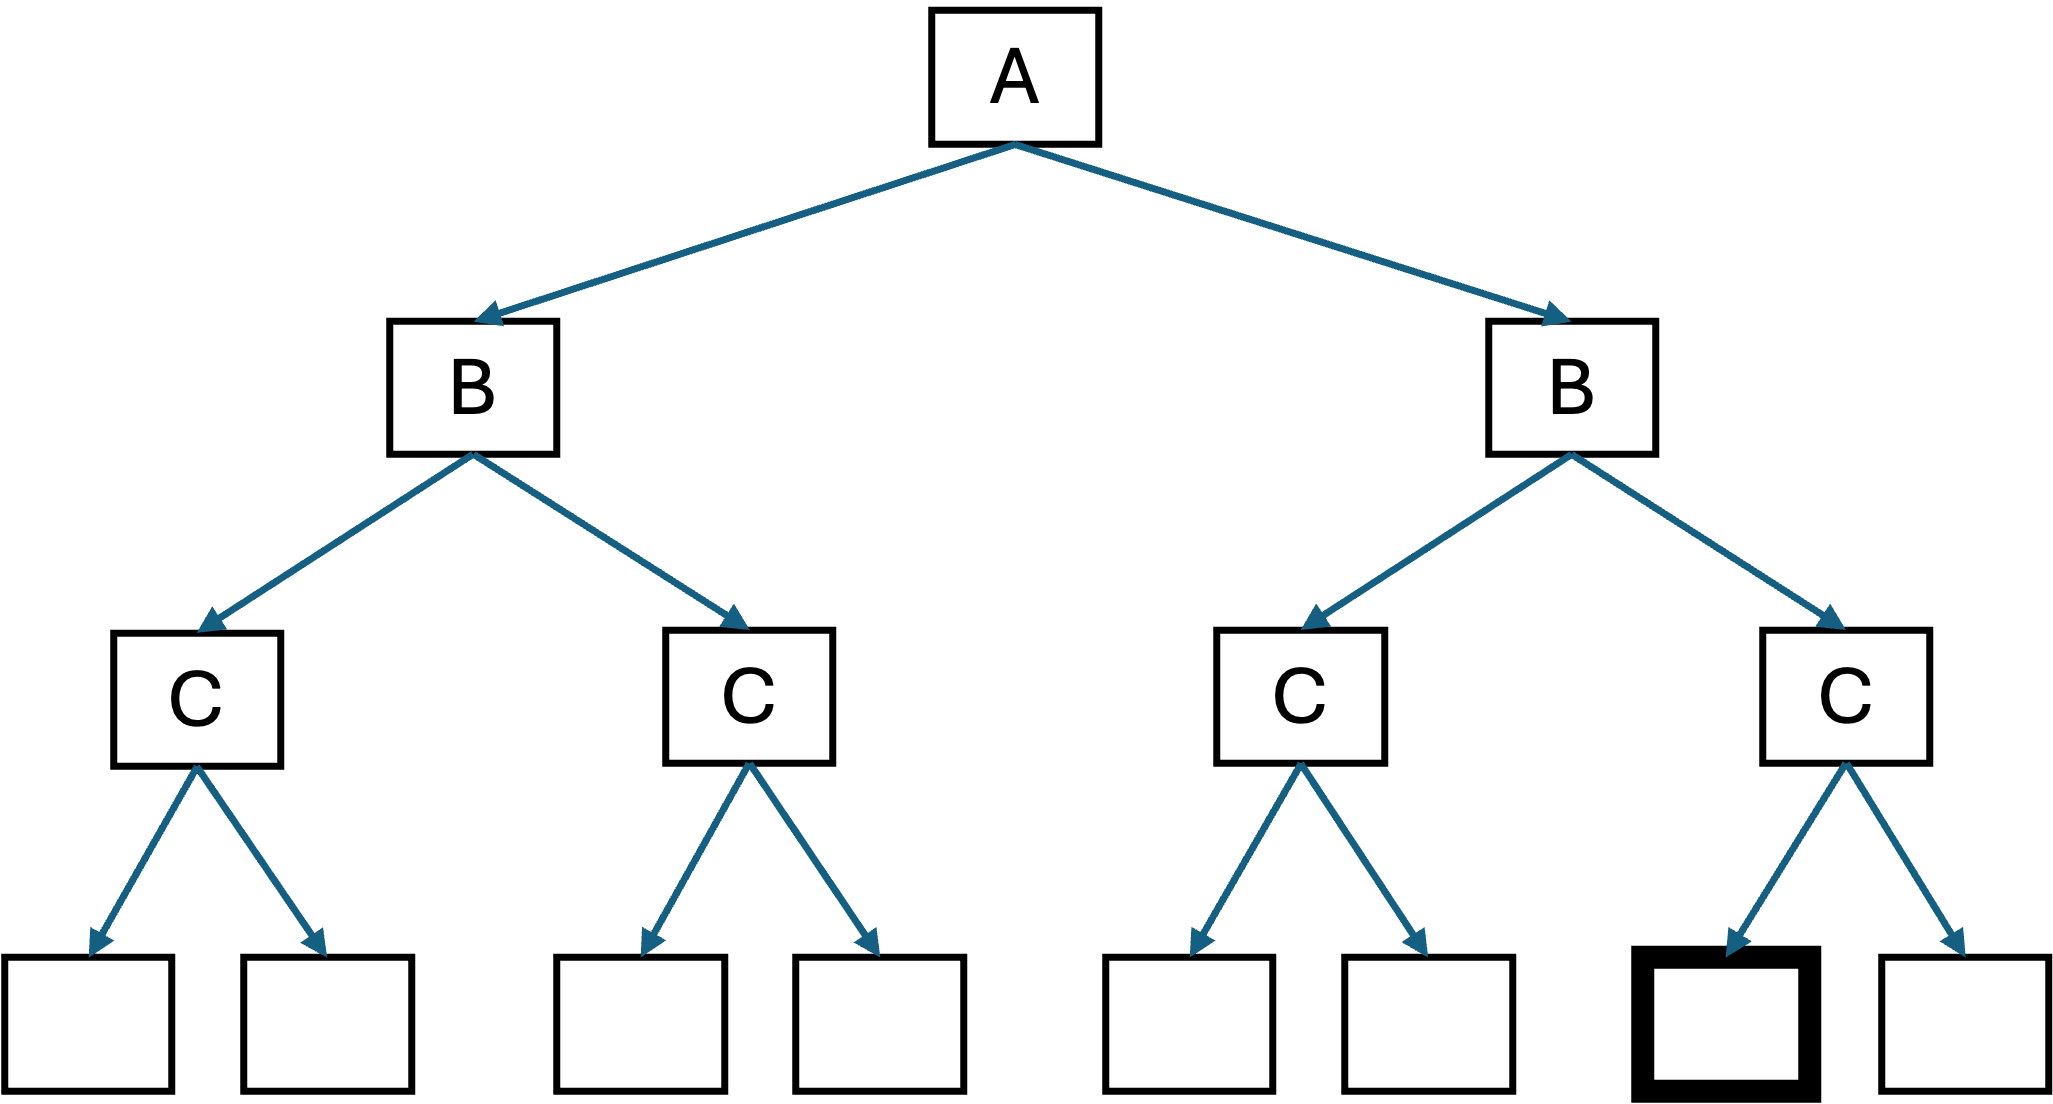
\includegraphics[width=2.5in]{alpha_beta_1.png}
\end{center}

\solutionspace{1cm}{15cm}{}
{\Foura}

\end{question}

\begin{question}[8] Game Tree 2

\begin{center}
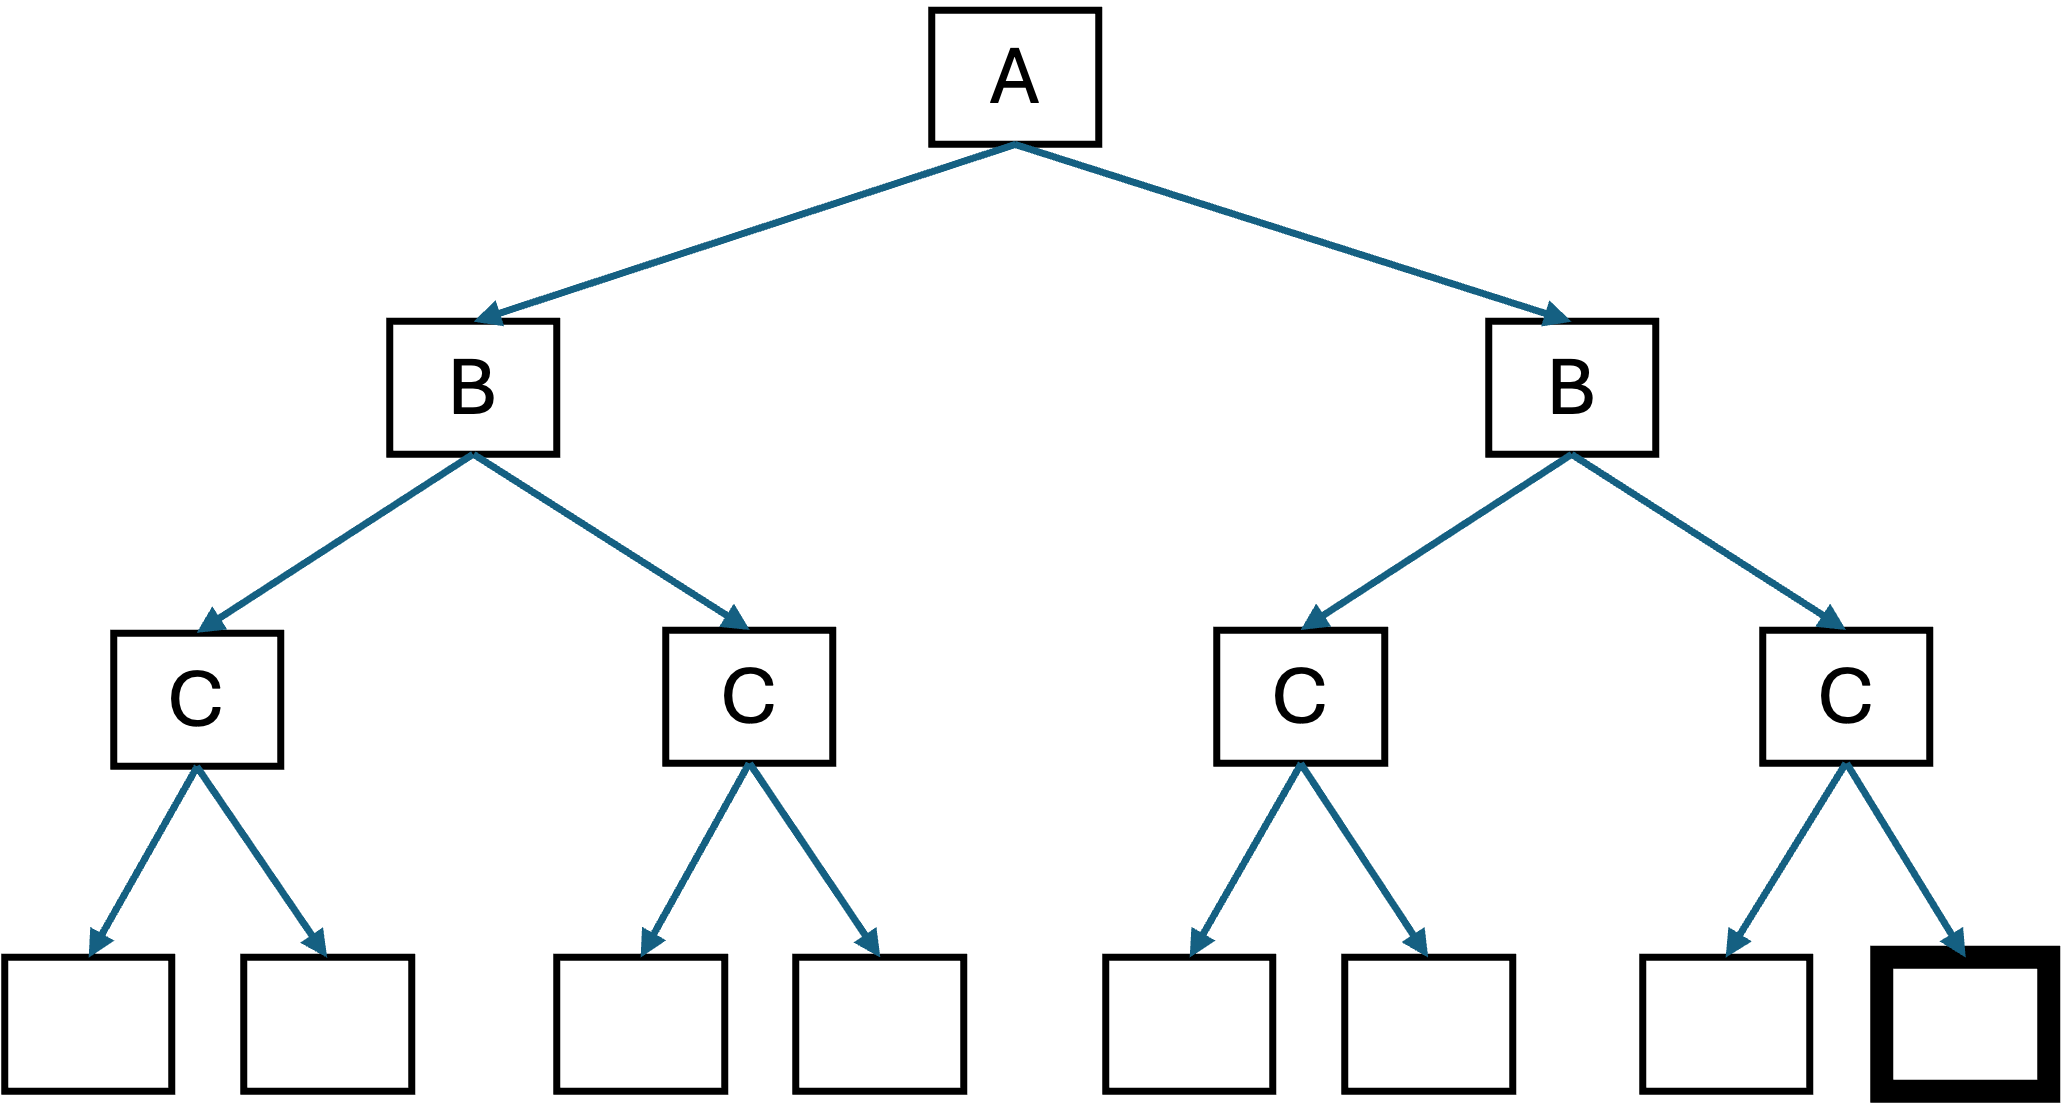
\includegraphics[width=2.5in]{alpha_beta_2.png}
\end{center}

\solutionspace{1cm}{15cm}{}
{\Fourb}

\end{question}

\begin{question}[8] Game Tree 3


\begin{center}
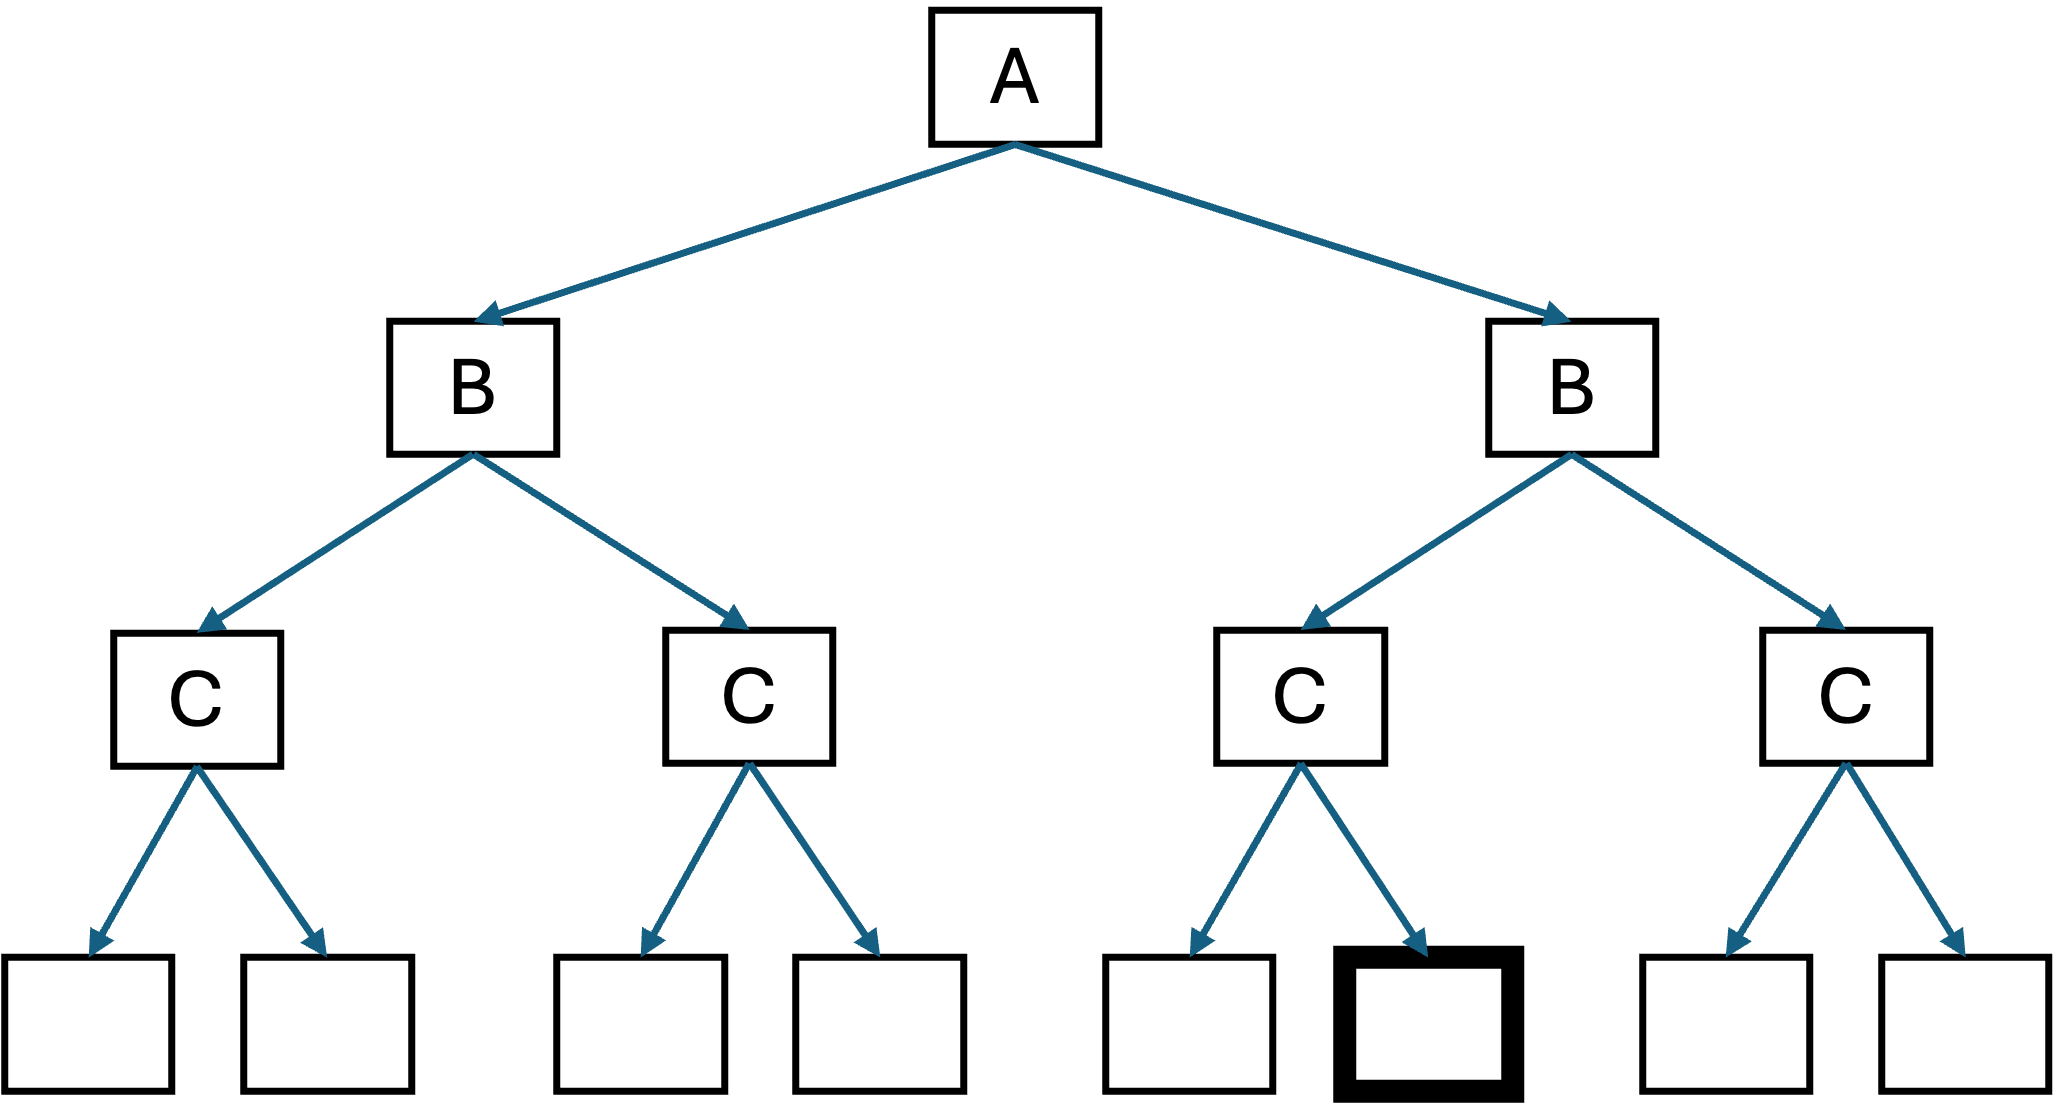
\includegraphics[width=2.5in]{alpha_beta_3.png}
\end{center}

\solutionspace{1cm}{15cm}{}
{\Fourc}

\end{question}

\end{problem}

\begin{problem}{Probability}

Consider the following probability tables for variables $A,B,C$.


\begin{center}
\begin{tabular}{ccc}
\begin{tabular}{|r|r|} \hline
A  & $P(A)$ \\ \hline
+a & 0.3      \\ \hline
-a & 0.7      \\ \hline
\end{tabular} &
\begin{tabular}{|r|r|r|} \hline
B  & A  & $P(B|A)$ \\ \hline
+b & +a & 0.7      \\ \hline
+b & -a & 0.6      \\ \hline
\end{tabular} & 
\begin{tabular}{|r|r|r|} \hline
C  & A  & $P(C|A)$ \\ \hline
+c & +a & 0.2      \\ \hline
+c & -a & 0.9      \\ \hline
\end{tabular}
\end{tabular}
\end{center}


\begin{question}[4] Derive $P(A,B)$ by filling in the entries below.  What formula are you using?

\begin{center}
\begin{tabular}{|r|r|r|} \hline
A  & B  & $P(A,B)$ \\ \hline
+a & +b &    \Fiveai     \\ \hline
+a & -b &   \Fiveaii       \\ \hline
-a & +b &    \Fiveaiii     \\ \hline
-a & -b &     \Fiveaiv    \\ \hline
\end{tabular}
\end{center}

\end{question}

\begin{question}[4] Derive $P(A|C)$ by filling in the entries below.  What formula are you using?

\begin{center}
\begin{tabular}{|r|r|r|} \hline
A  & C  & $P(A|C)$ \\ \hline
+a & +c &   \Fivebi      \\ \hline
+a & -c &   \Fivebii      \\ \hline
-a & +c &   \Fivebiii       \\ \hline
-a & -c &    \Fivebiv     \\ \hline
\end{tabular}
\end{center}

\end{question}

\begin{question}[8] Suppose $B$ and $C$ are conditionally independent given $A$.
  What is the formula you would use?  Then derive the full joint
  distribution $P(A,B,C)$ by filling in the entries below.

\begin{center}
\begin{tabular}{|r|r|r|r|l|l|} \hline
A  & B  & C  & $P(A,B,C)$ \\ \hline
+a & +b & +c &     \Fiveci       \\ \hline
+a & +b & -c &  \Fivecii          \\ \hline
+a & -b & +c &    \Fiveciii        \\ \hline
+a & -b & -c &   \Fiveciv         \\ \hline
-a & +b & +c &    \Fivecv        \\ \hline
-a & +b & -c &    \Fivecvi        \\ \hline
-a & -b & +c &    \Fivecvii        \\ \hline
-a & -b & -c &    \Fivecix       \\ \hline
\end{tabular}
\end{center}

\end{question}

\begin{question}[5] Use the full joint distribution you computed in problem 3 to derive the conditional distribution $P(A|+b,-c)$.  What formula
  would you use?  Then fill in the table below.  \\

\begin{center}
\begin{tabular}{|r|r|r|r|l|l|} \hline
A  & B  & C  & $P(A|+b,-c)$ \\ \hline
+a & +b & -c &    \Fivedi           \\ \hline
-a & +b & -c &    \Fivedii           \\ \hline
\end{tabular}
\end{center}

\end{question}



\end{problem}


\end{document}
